\documentclass{article}
\usepackage{anysize}
\marginsize{2.5cm}{1.8cm}{2.2cm}{2.5cm}
\usepackage[utf8]{inputenc}
\usepackage[T1]{fontenc}
\usepackage{graphicx}
\usepackage{url}
\pagestyle{empty}

\begin{document}
\begin{center}
\section*{FE\textsuperscript{2} Modeling of Liquid-Phase Sintering}
%
\begin{minipage}[t]{\textwidth}
\centering
\underline{Mikael Öhman}\textsuperscript{1}, Kenneth Runesson\textsuperscript{2},  Fredrik Larsson\textsuperscript{3}\\
\vspace{0.5cm}
\textsuperscript{1}Tillämpad Mekanik, Chalmers Tekniska Högskola, Göteborg, email: mikael.ohman@chalmers.se
\textsuperscript{2}Tillämpad Mekanik, Chalmers Tekniska Högskola, Göteborg, email: kenneth.runesson@chalmers.se
\textsuperscript{3}Tillämpad Mekanik, Chalmers Tekniska Högskola, Göteborg, email: fredrik.larsson@chalmers.se
\end{minipage}
\end{center}

\large
Please, write the title in: bold; capital letters. Underline the name of the author who will present the paper. The abstracts should be written in single-spaced A4 paper format (210 $\times$ 297 mm), with margins of 25 mm at left, right, top and bottom. The abstract is limited to one page. Figures can be included as Figure \ref{Figure1}. References should be included in \cite{Lars} style.

Separate paragraphs with an indentation. Equations should be centered and numbered consecutively with equation numbers in parentheses flush with the right margin, as in (\ref{eq1}). Shorter equations and mathematical expressions can be displayed in-line, provided that their formatting requirements do not disturb line spacing of the paragraph.
%
\begin{equation}\label{eq1}
\frac{\partial{\varphi}}{\partial{t}}+\frac{1}{2}\nu^2+\frac{p}{\rho}+gz=f(t)
\end{equation}
%
\begin{figure}[htb]
\begin{center}
\begin{minipage}[t]{.45\textwidth}
%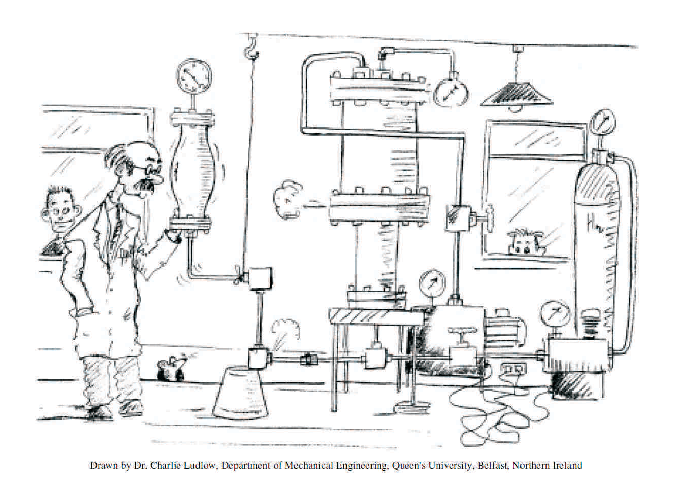
\includegraphics[width=\textwidth]{pic}
\caption{\footnotesize Example of a figure} \label{Figure1}
\end{minipage}
\end{center}
\end{figure}

The abstracts should be submitted electronically through the conference homepage, not later than 17 April 2011. Please convert your abstract to a pdf document and upload the pdf file only.
If you are also preparing an extended abstract it should follow the guideline given here.
\begin{thebibliography}{00}
\normalsize
 \bibitem{Lars}
   L. J. L. Nordström, H. Johansson, F. Larsson. A strategy for input estimation
   with sensitivity analysis. \emph{International Journal for Numerical Methods in Engineering}, 69 pp. 2219-2246, 2007.
 \bibitem{OOFEM}
  B. Patzák, OOFEM project home page, \url{http://www.oofem.org}, 2000.
\end{thebibliography}
\end{document} 